\documentclass{article}
\usepackage{graphicx}
\usepackage{natbib}
\usepackage{subfig}

\title{Phenomenological Robotics}
\author{Bruno Nery\\
        \texttt{bnery@isr.ist.utl.pt}}

\begin{document}

\maketitle

In the world of Good Old Fashioned Artificial Intelligence (GOFAI), scientists
attempted to fabricate intelligence by doing inference on symbolic
representations of the world. 

% 1.A. "Failure" of the computational hypothesis on everyday coping (being in
% the world is more basic than thinking).
% (Source: \cite{dreyfus07}.)

Dreyfus~\cite{dreyfus07} points out that the pioneers in GOFAI learned, directly
or indirectly, from the philosophers. Hobbes' claim that reasoning was
calculating and Descartes' mental representations, among others, are cited as
examples. At the same time, he states that the critical insights formulated by
existentialist philosophers, such as Heidegger and Merleau-Ponty, were a sign
that their enterprise was comdemned to failure. He affirms that

\begin{quotation}
  Heidegger's important insight is not that, when we solve problems, we
  sometimes make use of representational equipment outside our bodies, but that
  \emph{being-in-the-world} is more basic than \emph{thinking} and solving
  problems; that it is not representational at all.
\end{quotation}

% 1.?. On Brooks attempt. On Dreyfus believe on the failure of GOFAI and Brooks.

In Brooks' \cite{brooks91} approach, this is done by making agents respond to
fixed isolable features of the environment. Dreyfus \cite{dreyfus07} believes
that the basis of human intelligence, coping with everyday life, cannot be
achieved by any of the approaches described above. Instead, the fact that

\begin{quotation}
  \dots embodied beings like us take as input energy from the physical universe
  and respond in such a way as to open them to a world organized in terms of
  their needs, interests, and bodily capacities, without their minds needing to
  impose meaning on a meaningless given \dots nor their brains converting
  stimulus input into reflex responses \dots
\end{quotation}

% 1.C. Relation to affordances.
% (Source: Thesis journal, pages 130 to 139, 16/03/2011).
% Note: the following two paragraphs only introduce affordances and a reason
% for using it in robotics. Citing Chemero (2003) might be needed too. Examples
% of affordance based robotics (from Rome's book) should be in section 3.

Gibson~\cite{gibson1979} defines the \emph{affordances} of the environment as

\begin{quotation}
  \dots what it \emph{offers} the animal, what it \emph{provides} or
  \emph{furnishes}, either for good or ill. \dots [S]omething that refers to
  both the environment and the animal \dots.
\end{quotation}

Rome, Hertzberg and Dorffner~\cite{rome2008}, in their preface to ``Towards
Affordance-Based Robot Control'', affirm that the concept of affordance has
rarely been used in robotics or artificial intelligence, despite the original
perspective it offers on coupling perception, action and reasoning.

% 1.E. Robots have different bodies, different perceptions and different needs
%      from ours.
% (Source: Thesis journal, pages 006 to 015, 14/12/2010).
% Note: it might make more sense to propose the importance of the robots' bodies
% after introducing Todes (section 3.A). I'm not sure, however, of how to
% restructure the text to accomplish that.

Each robot has a different body, consisting of a set of sensors and actuators. 
For this reason, a robot experiences the world in a very specific way. Its body
defines not only what it can do, but also the way in which it sees the world.
Take the HERB~\cite{srinivasa2009herb}, the iCub~\cite{metta2010icub}, and the
Pioneer P3-DX robots, for example, depicted in
Figure~\ref{fig:herb_icub_pioneer}.

\begin{figure}[h]
  \centering
  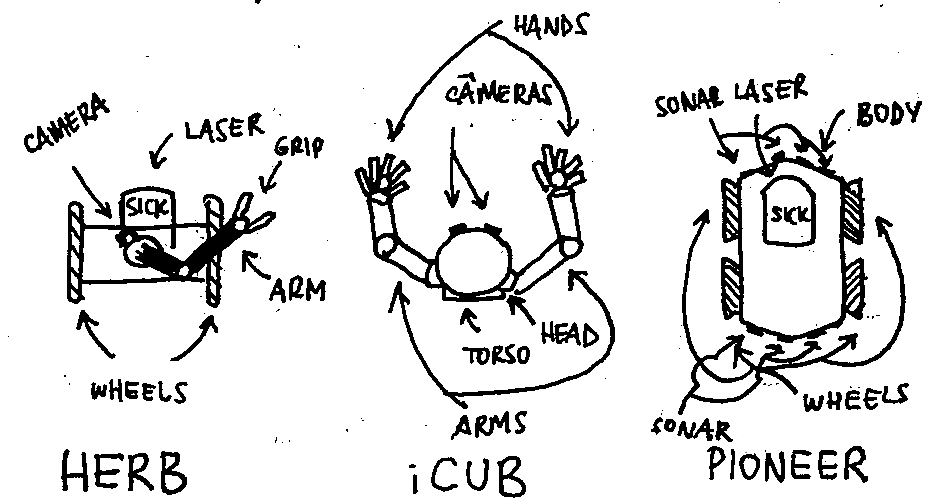
\includegraphics{figures/herb_icub_pioneer.png}
  \caption{HERB, iCub, and Pioneer P3-DX robots}
  \label{fig:herb_icub_pioneer}
\end{figure}

The HERB sees the world in \emph{forward mode} through its laser range finder
and its camera, coupled with its body movement. The iCub, in its
\emph{paraplegical} version, can only see the world in a left-to-right (and
right-to-left) manner through its cameras and head/torso movement. It can also
grasp nearby objects in order to examine them better. Finally, the Pioneer P3-DX
experiences the world in two different directions at the same time through its
sonars and its wheels movement. 

% 2. Relation between phenomenology and alternative psychology theories.

\section{Phenomenology and psychology theories}

% 2.B. Merleau-Ponty skills (refined situations) vs. Eleanor Gibson.
% (Source: Thesis journal, pages 140 to 149, 29/03/2011).
% (Source: \cite{gibson2000}.)

Dreyfus~\cite{dreyfus2002} shows that learning and skillful action, deemed as
basic forms of intelligent behavior, can be explained without recurring to
mental representations. To accomplish this, he explains the two central concepts
in Merleau-Ponty's \emph{Phenomenology of Perception}:

\begin{itemize}
\item \textbf{intentional arc:} is the strong connection between an agent and
its environment. In that sense, the skills learned by an agent are not kept as
representations in the mind, but as dispositions to respond to solicitations of
situations in the environment;
\item \textbf{maximal grip:} is the tendency of an agent to respond to these
solicitations in a way that brings the situation status closer to what it
considers optimal.
\end{itemize}

Gibson and Pick~\cite{gibson2000} propose that the process of learning is one of
discrimination rather than association, that is, through the refinement of the
sensorimotor knowledge acquired through the selection of patterns in our
interaction with the world. According to them, this selection process happens
based on two criteria:

% (\cite{gibson2000}, pages 154-156).

\begin{itemize}
\item \textbf{affordance fit:} what increases the fit between the organism and
its environment, according to its capacities and goals;
\item \textbf{economy:} what reduces the need for action and perceptual
information to accomplish a given task. -- optimization
\end{itemize}

These criteria can be seen as directly related to Merleau-Ponty's
\emph{intentional arc} and \emph{maximal grip}, respectively.

% 2.C. Merleau-Ponty vs. Coupling (van Gelder) vs. Stepp vs. Freeman.
% (Source: Thesis journal, pages 124 to 129, 11/03/2011).
% (Source: Thesis journal, pages 90 to 99, 18/02/2011).
% Note: Van Gelder ``coupling'' seems to be directly related to Freeman's basins
% of attraction. I don't see how Stepp would come between them. 2.D is supposed
% to be EST vs. discrete basin transitions, so it might belong down there. Maybe
% we could cite our work on EST that also includes coupling.

Van Gelder~\cite{vangelder1998} defends the \emph{dynamical hypothesis} in
cognitive science, stating that

\begin{quotation}
  \dots cognitive agents ``are'' \dots not some particular dynamical systems but
  as many systems as are needed to produce \dots cognitive performances \dots
\end{quotation}

He proposes that a cognitive system interacts with the environment through
\emph{coupling}, with input influencing the direction of change continuously and
output doing the same to the external world. Two different systems forging each
other's transformations at the same time.

Freeman~\cite{freeman1991}, after a set of experiments with rabbits, developed
an \emph{attractor theory}, where the brain can be understood as a dynamical 
system. According to this theory, the brain is composed of a set of energy peaks
and valleys (formed from one's past experiences). When the subject is in a
specific type of situation, the corresponding part of the brain landscape is
activated, and movements are caused to get the brain closer to a state of
minimum energy, called a ``basin of attraction''.

% 2.D. EST vs. Freeman (discrete basin transitions).
% (Source: our BICA10 paper).
% (Source: our Paladyn paper).
% Note: I didn't make the comparison with the discrete basin transitions from
% Freeman here because I believe it would belong together (and better) in the
% end of the section.

Event Segmentation Theory provides a model of how the human brain segments
perception into a sequence of events~\cite{kurby07,zacks07}. This model sustains
that event segmentation is based on the detection of prediction errors in the
sensory stream. In particular, the human brain is permanently making predictions
and comparing them with the actual outcome. Events are detected whenever a
significant disparity between prediction and outcome is encountered.

Nery and Ventura~\cite{nery2011} address the problem of segmenting a robot's
perception into meaningful events, based on Event Segmentation Theory. In this
approach, the prediction of the environment evolution is done using a dynamical
systems approach, where the predictor system has a delayed coupling with the
environment.

% 2.E. Merleau-Ponty (demand) vs. Chemero
% (Source: Thesis journal, pages 100 to 109, 03/03/2011).

Chemero~\cite{chemero2003} criticizes Gibson's original definition of
affordances, deeming it as deceitful. He defends that the perception of the
environment is always connected to the animal, calling the perceived items
\emph{features of situations}. He points out that are not directly related to
``body scale'', but rather to the animal's ``abilities'', arguing that these are
functional properties of the animal that happened to be historically useful.

Chemero defines organisms as ``ability sets'' (and some abilities depend on
others to function, e.g., walking depends on standing). Which abilities can be
used depend on the current situation. He defends that an ``affordance layout''
exists, and that this layout is changed by ``events''.

% Note: The paragraph below tries to put together everything that was described
% above: Van Gelder's coupling is the intentional arc; Freeman's basis of
% attraction implement the maximal grip. Our work connects events and coupling,
% justifying the corroboration of events to Chemero's affordance layout and its
% changes caused by ``events''. Finally, Chemero's concept of affordances itself
% can be seen as an instance of the intentional arc (opportunities presented by
% the environment that ``call us'' to act on it), but on a different timescale.

Van Gelder's idea of a cognitive system being direcly connected to the world can
be seen as an instance of Merleau-Ponty's \emph{intentional arc}, where
Freeman's results support the validity of the \emph{maximal grip} concept.
The work of Nery and Ventura shows the connection between the segmentation of
perception into events and the eventual coupling of an organism and its
environment. Chemero's idea of events changing the layout of affordances is
corroborated by Event Segmentation Theory. The way Chemero presents the
concept of affordances reinforces the idea of \emph{intentional arc}, closing
the loop.

% 3. In Robotics, Phylosophy and Related Work.

\section{Phenomenology and robotics}

% 3.A. Kuipers vs. Todes.
% (Source: \cite{todes2001}, page xix).
% (Source: Thesis journal, pages 42 to 42, 05/01/2011).

Dreyfus, in his introduction to Todes' \emph{Body and World}~\cite{todes2001},
describes the fundamental role played by the body in structuring the
spatiotemporal field that defines human experience

\begin{quotation}
  \dots the structure of the active body produces our unified experience of
  space and time. Since the body moves forward more effectively than backwards,
  it opens a \emph{horizontal field} that organizes experience in what can be
  coped with directly, what can be reached with effort, and what is over the
  perceptual horizon. Furthermore, the front/back asymmetry of the active body
  \dots organizes the temporal field.
\end{quotation}

% Reviewing Dreyfus introduction to Todes' Body and World, I realized that his
% work contributes a lot more than just the importance of the body and its
% orientation. According to Dreyfus, he goes further on improving the concepts
% of intentional arc and maximal grip from Merleau-Ponty. It might be an
% interesting source of ideas, but I'm not sure they would fit in this text.

Pierce and Kuipers~\cite{pierce1997} developed an algorithm to obtain a robot's
perception model and its possible actions in an unknown environment. Despite the
importance given to the robot's body, they make a clear distinction between the
mind (agent) and the body (robot), seeing the first as learning to control the
second.

% Not present in the outline: Spinozism and how it counters Pierce and Kuipers.
% I'm not sure if the way the text below is structured adds much to the point.
% (Source: \cite{lemmen1997}).
% ATTENTION: I had access to this thesis via Porfirio Silva, who downloaded it
% from the author's website in 2002 (no longer available). According to his
% note, the author asks not to be cited without permission. I found no trace of
% the author online, with the exception of a paper from 1996 with the email
% ronaldl@cogs.susx.ac.uk. Chapters 6 and 7 might be worth a full read, as they
% verse on ``(Artificial) Life and Dynamical Theory'' and on ``Body and Soul''
% (``Non-Cartesian Robots'').

Lemmen~\cite{lemmen1997} developed what he called a ``Spinozist'' framework for
understanding cognition. Rooted on the work of Merleau-Ponty, one of its main
points is the proposal of leaving Cartesianism behind, stating that

\begin{quotation}
  For the Spinozist, mind and body form a concrete unity.
\end{quotation}

% 3.B. Affordances vs. Robotics (Rome's book).
% (Source: Thesis journal, pages 130 to 139, 16/03/2011).
% Note: I believe citing examples of affordances in Robotics is a must here.
% A bridge between the former subject (Todes-Kuipers-Lemmen) might be necessary,
% or even a new section.

% Note: the next reference being focused on the coupling between more than one
% robot, I'm not sure it fits completely here (in affordances) instead of
% somewhere else (in coupling) or nowhere at all.
Hafner and Kaplan~\cite{hafner2008} present the concept of \emph{interpersonal
maps}, creating a representation space that allows one's behavior to the
behavior of others. To validate their approach, they perform a set of
experiments with four-legged robots either acting alone or engaged in imitation.

Hertzberg et al.~\cite{hertzberg2008} discuss the perception of
\emph{navegability} as an affordance. He presents \emph{navegability maps} as an
example, and classify them as \emph{semantic maps}. They defend that

\begin{quotation}
  [E]very efficient robot control system includes highly tuned sensor data
  processing modules \dots to perceive \dots robot-environment relations that
  are necessary for the robot's intended function.
\end{quotation}

They leave, however, the insight to develop each of this processing modules to
the designer, making it impractical for robots that should work in unstructured,
dynamic environments.

Raubal and Maratz~\cite{raubal2008} propose a functional model based on an
extended theory of affordances. They demonstrate its applicability with two
different robot scenarios, where the objects ``tell'' the robot what they can be
used for. 

Sutton and Start~\cite{sutton2008} implement a system that segments images in
\emph{affordances} instead of \emph{objects}. The training dataset is labeled is
labeled manually. Even though, their algorithm is able to evaluate if a surface
``provides stable support'' (like a chair), ``confirms graspability'' (like any
graspable object) or ``confirms containment'' (like a cup). One of their results
worth mentioning is the labelling of an upside-down garbage can as ``sittable''.

Moratz and Tenbrink~\cite{moratz2008} discuss advances in \emph{spatial
cognition} and develop a method that allows a robot to acquire knowledge through
its interaction with a human. They also present an object recognition system
based in \emph{affordances}, but do not provide detailed on the matter.

Paletta and Fritz~\cite{paletta2008} describe a process of \emph{affordance
cueing} where a robot obtains a probability distribution over the possible
affordances from a set of features. They apply it to a scenario where a robot
interacts with magnetizable cans that might afford ``lifting'', using
Reinforcement Learning and Markov Decision Process to learn which features
might indicate the ``liftability'' of an object.

% 4. The IKEA scenario.
% (Source: Thesis journal, pages 130 to 139, 17/03/2011).

\section{The IKEA scenario}

\begin{quotation}
  A hammer is for hammering.
\end{quotation}

If you have a nail nearby, that might be the case. If you are assembling IKEA
furniture outdoors, however, a hammer might as well be ``for paper weighting''.
In the same sense, a ladder is only ``for climbing'' when you have the need to
reach a high place. Most of the times, a ladder will be
``for being in the way''.

Also, screwdrivers are, supposedly, ``for driving screws''. But what happens
when you a have a flat screwdriver and need to drive a Phillips-head screw
(Figure~\ref{fig:ikea_flat_phillips})? It is harder to drive it, but have you
ever tried driving a flat head screw with a Phillips screwdriver
(Figure~\ref{fig:ikea_phillips_flat})? It won't work, and you'll start asking
yourself what is wrong, and what you can do to fix it.

\begin{figure}[h]
  \centering
  \subfloat[][Flat screwdriver vs. Phillips-head screw] {
    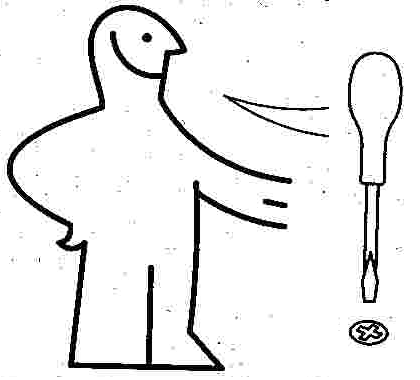
\includegraphics{figures/ikea_flat_phillips.png}
    \label{fig:ikea_flat_phillips}
  }
  \qquad
  \subfloat[][Phillips screwdriver vs. Flat head screw] {
    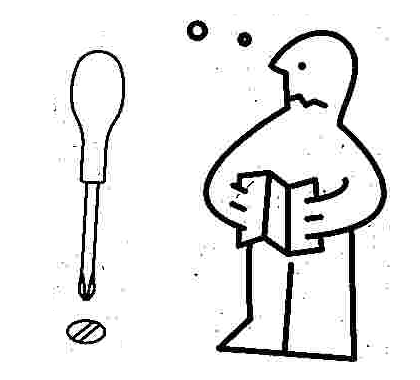
\includegraphics{figures/ikea_phillips_flat.png}
    \label{fig:ikea_phillips_flat}
  }
  \caption{The IKEA scenario}
\end{figure}

You will be having a breakdown, as described by Heidegger~\cite{dreyfus07}, and
the screwdriver will cease to be \emph{ready-to-hand} and become
\emph{present-at-hand} until you can figure out the problem. But how do we equip
a robot with the same capabilities so that it can function in a human world?

% Not present in the outline: learning process in infancy. This might not be the
% best place for this part, but it definitely goes together with the
% cornerstones of the framework below.
% (Source: Thesis journal, pages 140 to 149, 28/03/2011).
% (Source: \cite{gibson2000}, pages 134 to 149, chapter 8).

Gibson~\cite{gibson2000} affirms that perceptual learning predates birth. She
describes a number of cases, going from early perceptual learning to elaborate
sequences of action in older infants. In these cases, the infant learns:

\begin{itemize}
\item about oneself;
\item to control an event;
\item to perceive an unitary object;
\item what happens next in an observed event;
\item to participate in a communicative event;
\item to differentiate multimodally specified events;
\item distinctive features of things;
\item to use an object or an act as means;
\item about causal relations in observed events.
\end{itemize}

% Not present in the outline: cornerstones of the framework. This might not be
% the best place for this part.
% (Source: Thesis journal, pages 100 to 109, 03/03/2011).

Before a robot is able to handle a breakdown, it needs to be able to function in
the world seamlessly, fullfiling its needs by executing one action after the
other, using what is available to it in a given moment. To be able to do that,
the following set of basic capabilities might be a good place to start:

\begin{itemize}
\item \textbf{body knowledge:} know its own body, be able to detect its current
state and how it changes according to its movements;
\item \textbf{skill acquisition:} know how discover and/or learn a set of
abilities that allow it to interact with the world;
\item \textbf{object detection:} know how to single out objects and detect
properties that allow it to use them in a particular manner.
\end{itemize}

\bibliographystyle{plain}
\bibliography{prsurvey}

\end{document}
